\documentclass{article}

%%%%%%%%%%%%%%%%%%%%%%%%%%%%%%%%
% PACKAGES
%%%%%%%%%%%%%%%%%%%%%%%%%%%%%%%%
\usepackage{times}
\usepackage{fullpage}
\usepackage{latexsym}
\usepackage{amsmath}
\usepackage{amssymb}
\usepackage{mathtools}
\usepackage{accents}
\usepackage{tikz}
\usepackage{pgfplots}
\usepackage[ruled]{algorithm}
\usepackage{algpseudocode}
\usepackage{dsfont}
\usepackage[bf]{caption}
\usepackage{hyperref}
\hypersetup{
    bookmarks=true,         % show bookmarks bar?
    unicode=false,          % non-Latin characters in AcrobatÕs bookmarks
    pdftoolbar=true,        % show AcrobatÕs toolbar?
    pdfmenubar=true,        % show AcrobatÕs menu?
    pdffitwindow=false,     % window fit to page when opened
    pdfstartview={FitH},    % fits the width of the page to the window
    pdftitle={My title},    % title
    pdfauthor={Author},     % author
    pdfsubject={Subject},   % subject of the document
    pdfcreator={Creator},   % creator of the document
    pdfproducer={Producer}, % producer of the document
    pdfkeywords={keyword1} {key2} {key3}, % list of keywords
    pdfnewwindow=true,      % links in new window
    colorlinks=true,       % false: boxed links; true: colored links
    linkcolor=red,          % color of internal links (change box color with linkbordercolor)
    citecolor=blue,        % color of links to bibliography
    filecolor=magenta,      % color of file links
    urlcolor=cyan           % color of external links
}
\usepackage{amsthm}
\usepackage{natbib}
\usepackage[capitalize]{cleveref}
\usepackage{graphicx}

%%%%%%%%%%%%%%%%%%%%%%%%%%%%%%%%
% MACROS
%%%%%%%%%%%%%%%%%%%%%%%%%%%%%%%%
\newcommand{\defined}{\vcentcolon =}
\newcommand{\rdefined}{=\vcentcolon}
\newcommand{\E}{\mathbb E}
\newcommand{\Var}{\operatorname{Var}}
\newcommand{\calF}{\mathcal F}
\newcommand{\sr}[1]{\stackrel{#1}}
\newcommand{\set}[1]{\left\{#1\right\}}
\newcommand{\ind}[1]{\mathds{1}\!\!\set{#1}}
\newcommand{\argmax}{\operatornamewithlimits{arg\,max}}
\newcommand{\argmin}{\operatornamewithlimits{arg\,min}}
\newcommand{\floor}[1]{\left \lfloor {#1} \right\rfloor}
\newcommand{\ceil}[1]{\left \lceil {#1} \right\rceil}
\newcommand{\eqn}[1]{\begin{align}#1\end{align}}
\newcommand{\eq}[1]{\begin{align*}#1\end{align*}}
\newcommand{\Ber}{\operatorname{Bernoulli}}
\renewcommand{\P}[1]{\operatorname{P}\left\{#1\right\}}


%%%%%%%%%%%%%%%%%%%%%%%%%%%%%%%%
% THEOREMS
%%%%%%%%%%%%%%%%%%%%%%%%%%%%%%%%
\theoremstyle{plain}
\newtheorem{theorem}{Theorem}
\newtheorem{proposition}[theorem]{Proposition}
\newtheorem{lemma}[theorem]{Lemma}
\newtheorem{corollary}[theorem]{Corollary}
\theoremstyle{definition}
\newtheorem{definition}[theorem]{Definition}
\newtheorem{assumption}[theorem]{Assumption}
\newtheorem{remark}[theorem]{Remark}
\newtheorem{example}[theorem]{Example}

\title{Intervention Bandits}
\author{Blah blah}

\begin{document}
\def\ci{\perp\!\!\!\perp}
\maketitle

\begin{abstract}
An abstract.
\end{abstract}

\section{Introduction}

Useful references are: \cite{BC12}.

\section{Notation}

Assume we have a known causal model with binary variables $\boldsymbol{X} = \{X_{1}..X_{K}\}$ that independently cause a target variable of interest $Y$. We can run sequential experiments on the system, where at each timestep $t$ we can select a variable on which to intervene and then we observe the complete result, $(\boldsymbol{X}_{t},Y_{t})$ This problem can be viewed as a variant of the multi-armed bandit problem.


Let $p \in [0,1]^K$ be a fixed and known vector. In each time-step $t$:
 
\begin{enumerate}
\item The learner chooses an $I_t \in \set{1,\ldots, K}$ and $J_t \in \set{0,1}$.
\item Then $X_t \in \set{0,1}^K$ is sampled from a product of Bernoulli distributions, $X_{t,i} \sim \Ber(p_i)$ 
\item The learner observes $\tilde X_t \in \set{0,1}^K$, which is defined by 
\eq{
\tilde X_{t,i} = \begin{cases}
X_{t,i} &\text{if } i \neq I_t \\
J_t & \text{otherwise}\,.
\end{cases}
}
\item The learner receives reward $Y_t \sim \Ber(q(\tilde X))$ where $q:\set{0,1}^K \to [0,1]$ is unknown and arbitrary.
\end{enumerate}
The expected reward of taking action $i,j$ is $\mu_{i,j} = \E[q(X)|do(X_i = j)]$. The optimal reward and action are $\mu^*$ and $(i^*,j^*)$ respectively,
where $(i^*,j^*) = \argmax_{i,j} \mu_{i,j}$ and $\mu^* = \mu(i^*,j^*)$. The $n$-step cumulative expected regret is
\eq{
R_n = \E \sum_{t=1}^n \left(\mu^* - \mu_{I_t,J_t}\right).
}

\section{Estimating $\mu_{i,j}$}
The most natural way to estimate $\mu_{i,j}$ is to compute an empirical estimate based on samples when that action was taken. This approach would
lead directly to the UCB algorithm with $2K$ actions and a regret bound that depended linearly on $K$. In this instance we can significantly
outperform this approach by exploiting the known causal structure of the problem.

\eq {
P(Y|do(X_i=j)) &= P(Y|X_i = j)\\
 &= \sum_{b}P(Y|X_i = j,X_a = b)P(X_a = b|X_i = j) \\
 &= \sum_{b}P(Y|X_i = j,X_a = b)P(X_a = b), \; \forall \, a \in \{1...K\}/i \text{ as } X_a \ci X_i\\
 &= \sum_{b}P(Y|X_i = j,do(X_a = b))P(X_a = b) 
}

Fix some time-step $t$ and $i \in \set{1,\ldots,K}$ and $j \in \set{0,1}$. 

Let $\hat{\mu}_a$ be an empirical estimator for $P(Y|do(X_i=j))$ obtained via marginalization over $X_a$.

\eq {
\hat{\mu}_a &=
\begin{cases}
\frac{m_{a,1}}{n_{a,1}}p_a+\frac{m_{a,0}}{n_{a,0}}(1-p_a) & \text{if } a \neq{i} \\
\frac{m_{i,j}}{n_{i,j}} & \text{if } a=i \\
\end{cases}\\
\text{where:}\\
m_{a,b}    &= \sum_{s=1}^t \ind{X_i = j, I = a,J = b, Y = 1}_s \\
n_{a,b}    &= \sum_{s=1}^t \ind{X_i = j, I = a,J = b}_s \\
}



This gives $K$ estimators $\{\hat{\mu_1}...\hat{\mu_K}\}$ to be pooled into a single estimator $\hat{\mu}$.

\eq {
\hat{\mu} &= \sum^{K}_{a=1}\eta_a\hat{\mu}_a=\eta_i \frac{m_{i,j}}{n_{i,j}}+ \sum_{a \neq i} \eta_a \left[p_a \frac{m_{a,1}}{n_{a,1}} + (1 - p_a) \frac{m_{a,0}}{n_{a,0}}\right]\\
\text{where:}\\
\eta_a     &= \frac{n_a}{\sum_{a=1}^K n_a} \text{ and } n_{i,j}=\begin{cases} 
n_{i,j} & \text{if } a = i \\
\frac{1}{2}\min\set{\frac{n_{a,1}}{p_a}, \frac{n_{a,0}}{1-p_a}}  & \text{otherwise}
\end{cases}
}

If $p$ is not known, these expression are unchanged except that $p_a$ is replaced with $\hat{p}_a$

\eq{
\hat{p}_a = \frac{\sum_{s=1}^{t} \ind{X_a=1,I \neq a}_s}{\sum_{s=1}^{t} \ind{I \neq a}_s}
}

\begin{theorem} With probability at least $1 - \delta$ we have that:
$\displaystyle \left|\hat{\mu}_t - \mu\right| \leq \sqrt{\frac{\beta}{\sum_{a} n_a} \log{1 \over \delta}}$,
where $\beta > 0$ is some constant.
\end{theorem}

\begin{proof}
First note that $n_{a,b}$ is a random variable that is bounded by $t$ for all $a,b$.
We use the short-hand $\mu^{a,b}_{i,j} = \E[q(X) | X_i = j, X_a = b]$. Then
\eq{
\mu_{i,j} = p_a \mu_{i,j}^{a,1} + (1 - p_a) \mu_{i,j}^{a,0}\,.
}
Now we can apply Hoeffding's bound and the union bound to show that
\eq{
\P{\left|\frac{m_{a,b}}{n_{a,b}} - \mu_{i,j}^{a,b}\right| \geq \sqrt{\frac{1}{2n_{a,b}} \log \frac{4t}{\delta}}} \leq \frac{\delta}{2}\,.
}
Therefore by the union bound
\eq{
\P{\left|p_a \frac{m_{a,1}}{n_{a,1}} + (1 - p_a) \frac{m_{a,0}}{n_{a,0}} - \mu_{i,j}\right| \geq p_a \sqrt{\frac{1}{2n_{a,1}} \log\frac{4t}{\delta}}
+ (1 - p_a) \sqrt{\frac{1}{2n_{a,0}}\log\frac{4t}{\delta}}} \leq \delta\,
}
Now by Jensen's inequality 
\eq{
p_a \sqrt{\frac{1}{2n_{a,1}}\log\frac{4t}{\delta}} + (1 - p_a) \sqrt{\frac{1}{2n_{a,0}}\log\frac{4t}{\delta}}
&\leq \sqrt{\left(\frac{p_a}{2n_{a,1}} + \frac{1-p_a}{2n_{a,0}}\right)\log \frac{4t}{\delta}} \\
&\leq \sqrt{\max\set{\frac{p_a}{n_{a,1}}, \frac{1-p_a}{n_{a,0}}} \log\frac{4t}{\delta}} \\
&= \sqrt{{1 \over 2n_a} \log\frac{4t}{\delta}}\,.
}
Similarly,
\eq{
\P{\left|\frac{m_{i,j}}{n_{i,j}} - \mu_{i,j}\right| \geq \sqrt{\frac{1}{2n_a} \log\frac{4t}{\delta}}} \leq
\P{\left|\frac{m_{i,j}}{n_{i,j}} - \mu_{i,j}\right| \geq \sqrt{\frac{1}{2n_a} \log\frac{2t}{\delta}}} \leq \delta\,.
}
\end{proof}

\section{Algorithm}

\begin{algorithm}
\caption{UCB}
\begin{algorithmic}[1]
\State {\bf Input:} Number of variables $K$, vector $p \in [0,1]^K$, horizon $n$
\For{$t \in 1,\ldots,n$}
\For{$i \in 1,\ldots,K$}
\For{$j \in \set{0,1}$}
\State Compute $\tilde \mu_{i,j} = \hat \mu_{i,j} + \sqrt{\frac{\alpha}{\sum_{a} n_a} \log n}$ 
\EndFor
\EndFor
\State Choose $I_t, J_t = \argmax_{i,j} \tilde \mu_{i,j}$
\EndFor
\end{algorithmic}
\end{algorithm}

\section{Theorems}
\section{Experiments}



\begin{figure}[h]
\caption{Comparison of the performance of standard UCB versus causal UCB with $\beta=3$ and $\beta = 5$. 100 simulations were run for each algorithm up to a horizon of $10^5$ per value of $K$. Error bars span the 1st to 3rd quantile of the regret, round points mark the median and triangular points show the mean. For standard UCB the regret increases linearly with the number of arms $K$. For causal UCB the increase is sub-linear. Increasing $\beta$ leads to slower convergence but lower variance.}
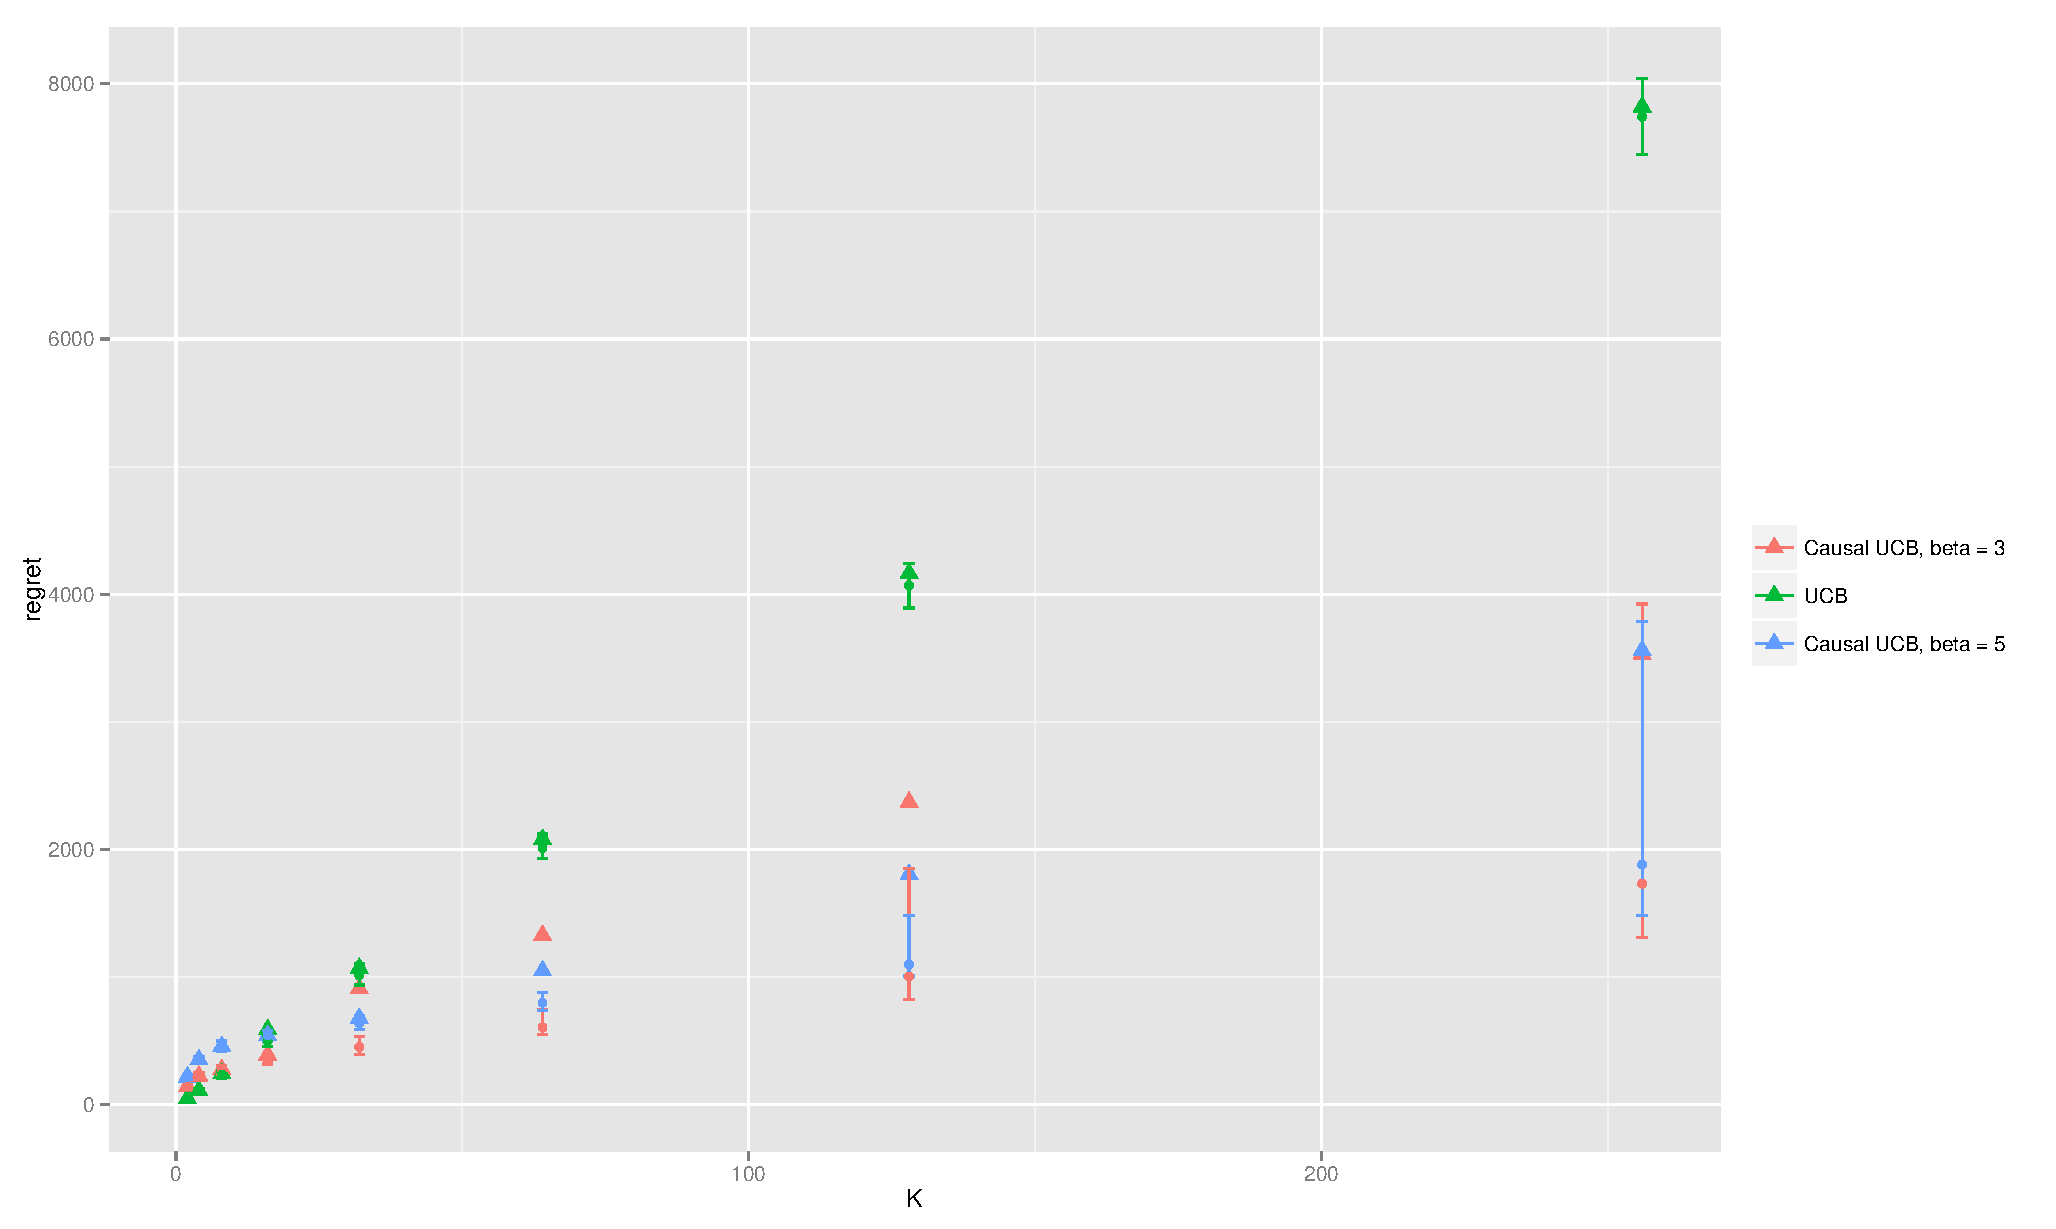
\includegraphics[width=1\textwidth]{regret_vs_K_series_beta.pdf}
\end{figure}

\begin{figure}[h]
\caption{The distribution of regret varies with the $\beta$ parameter in the bound in the estimator. As beta increases, the mean regret increases but the variance decreases. The plot shows the results of running $100$ independent bandits, with $K=256$ and $\epsilon=0.1$, up to a horizon $h=10^5$ for each value of $\beta$. }
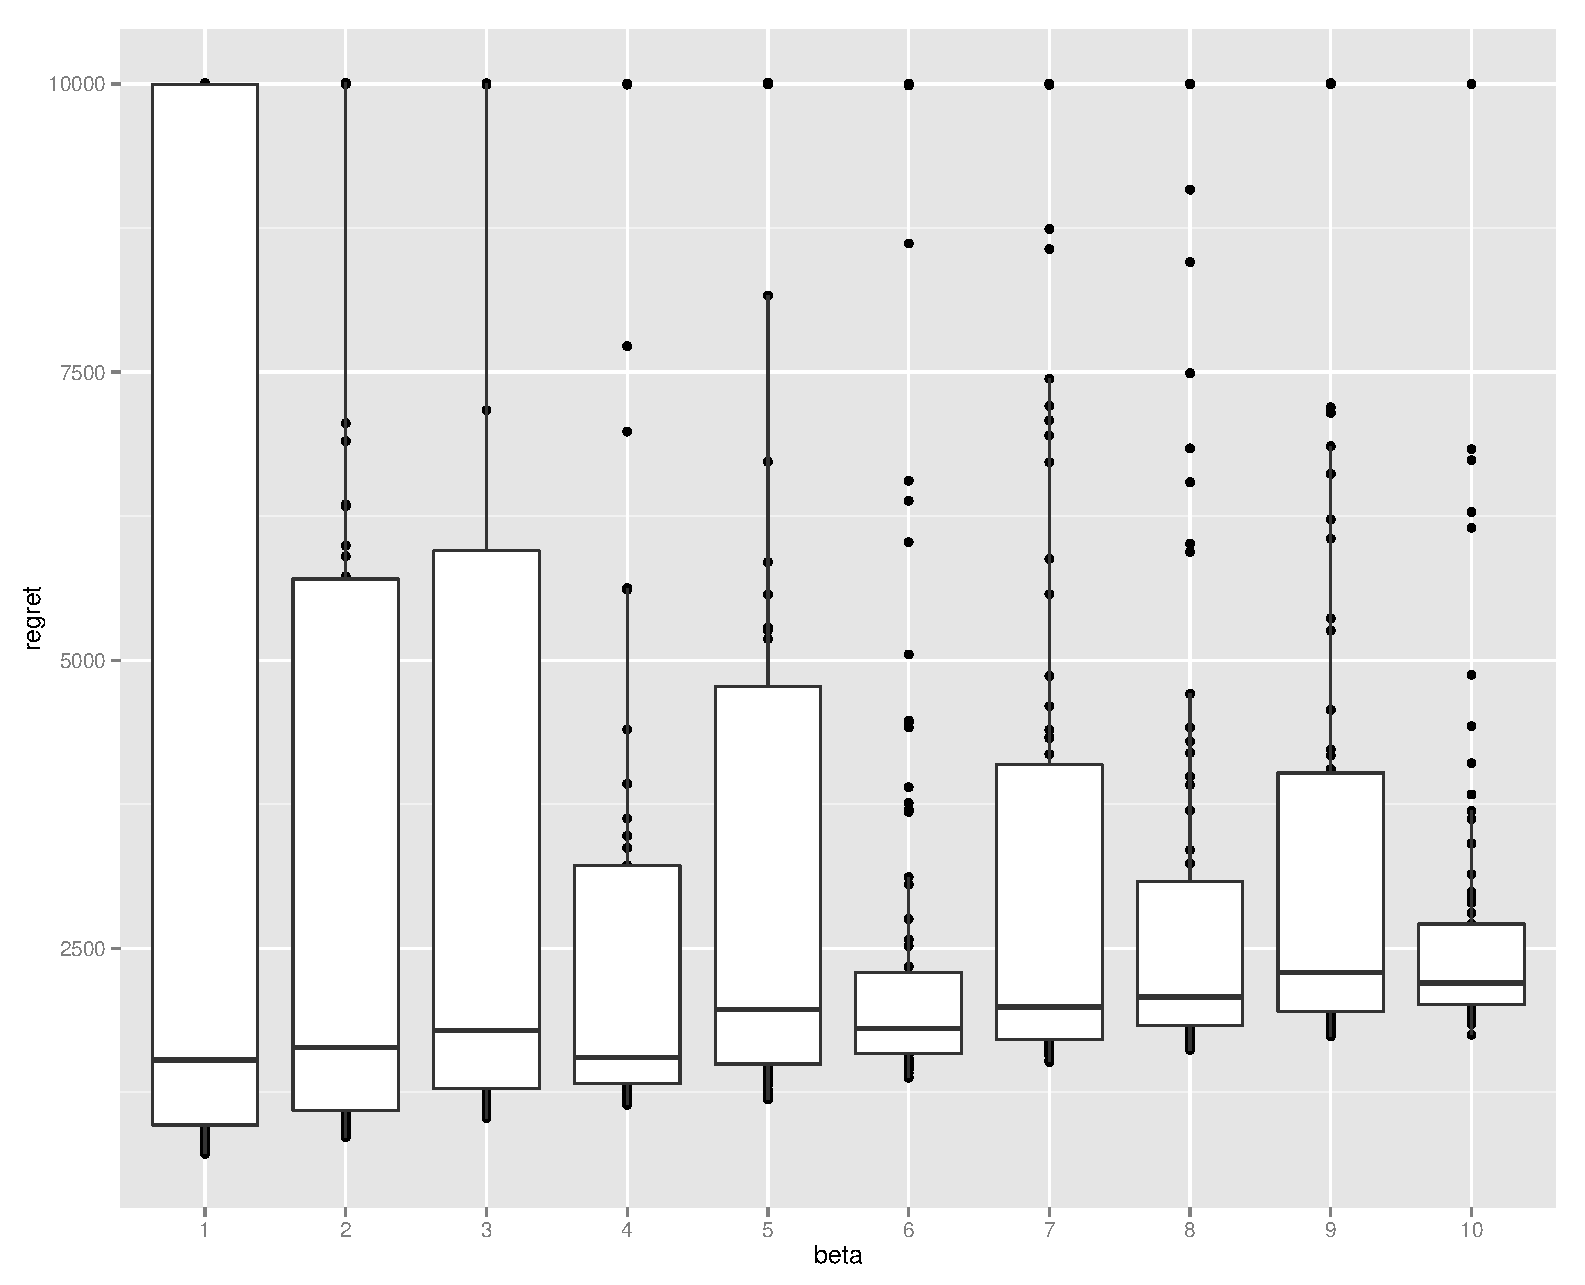
\includegraphics[width=0.7\textwidth]{regret_vs_beta_boxplot.pdf}
\end{figure}



Simululations to compare the performance of standard UCB with our modified algorithm. For each number of arms, $100$ bandits of each type were created and run upto to a horizon of $1000$ timesteps. The mean regret and its standard error from these simulations is plotted in figure \ref{fig:regretvsarms} The true data was generated from a model where:

\eq{
&p = [0.5]^{K}\\
&q(\boldsymbol{X}) = \begin{cases}0.5 & \text{if $X_{1}=0$}\\ 0.6 & \text{otherwise} \end{cases}
}






\section{Conclusion}

\bibliographystyle{plainnat}
\bibliography{c-bandit}

\end{document}



\begin{figure}[h]
\caption{Testing values of beta - 100 experiments for each value of beta, with a 4 armed bandit.}
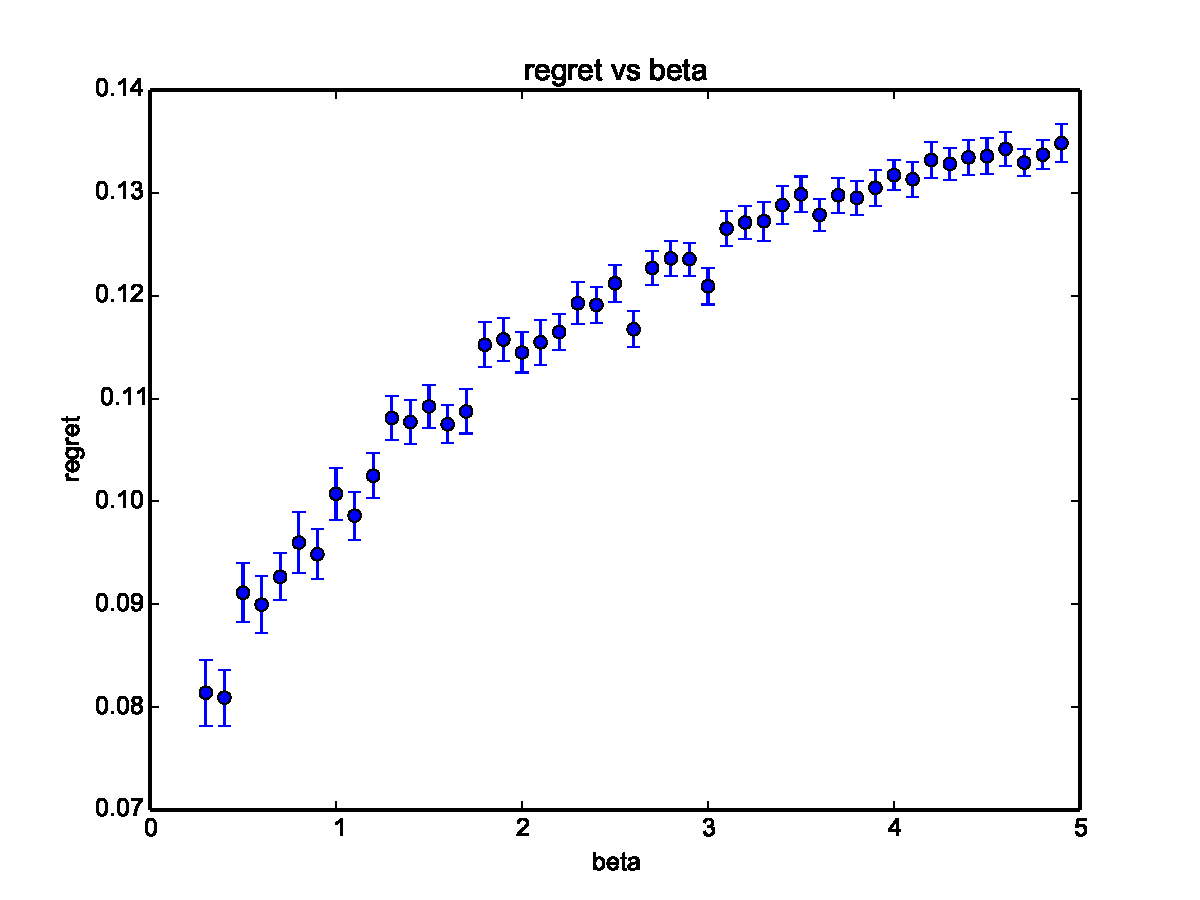
\includegraphics[width=0.7\textwidth]{regretvsbeta.pdf}
\end{figure}

\begin{figure}[h]
\caption{Shows relationship between the regret and the number of bandit arms $2K$ for the standard UCB algorithm and our modified algorithm.  }
\label{fig:regretvsarms}
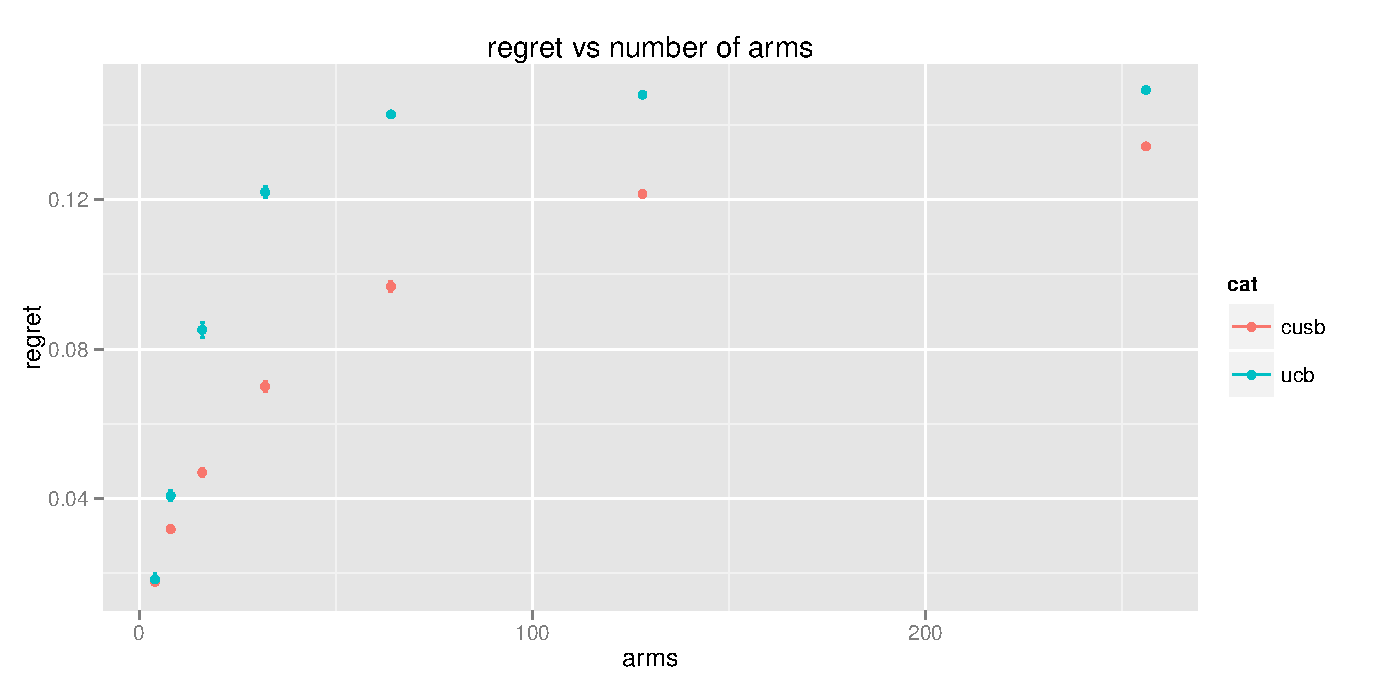
\includegraphics[width=0.9\textwidth]{regretvsarms.pdf}
\end{figure}

\begin{figure}[h]
\caption{Regret vs number of arms with horizon $100$}
\label{fig:regretvsarmsshorthorizon}
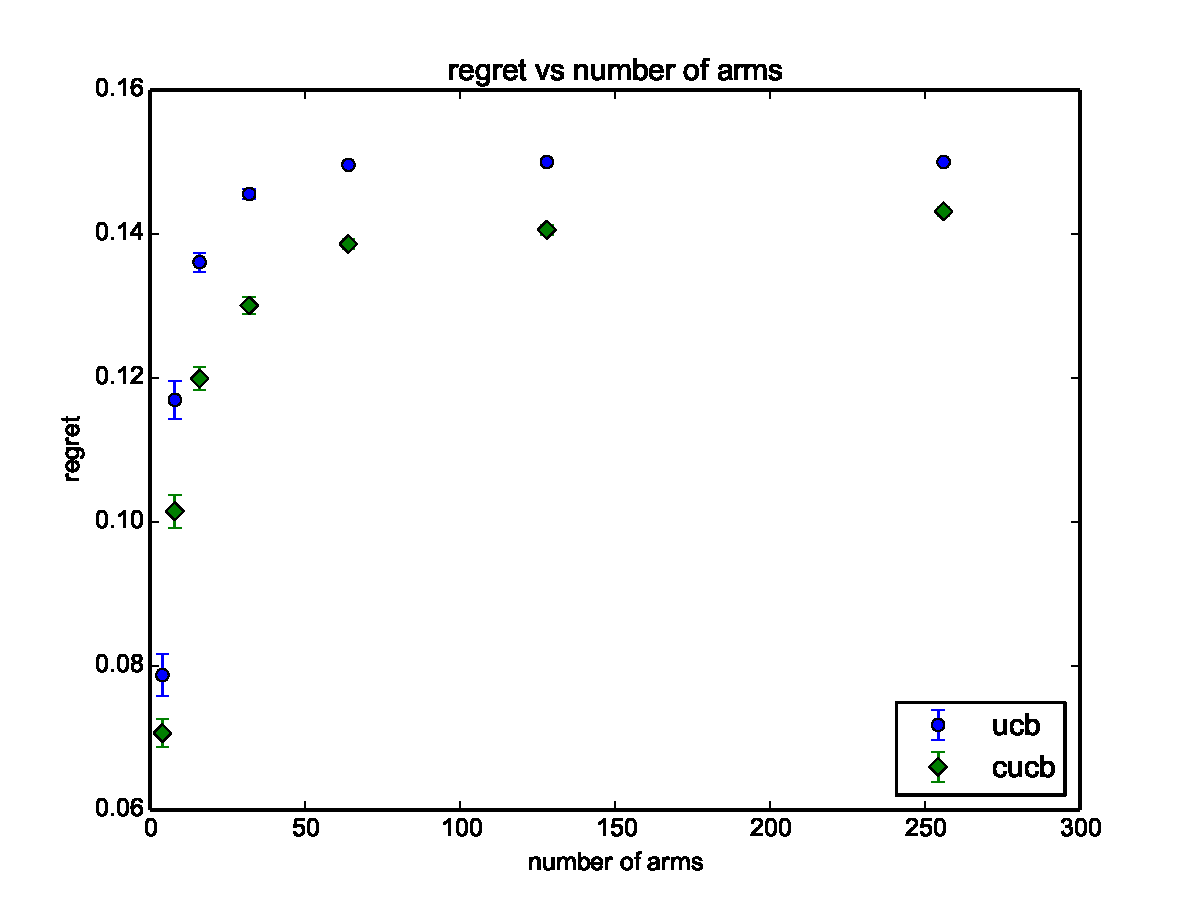
\includegraphics[width=0.8\textwidth]{regregvsamrs100.pdf}
\end{figure}

